% Gemeinsame Präambel für Spickzettel.tex, Spickzettel_mit_Hypothesentest.tex und Digital.tex
% Essential packages
\usepackage{fontspec} % For LuaLaTeX/XeLaTeX
\setmainfont{Latin Modern Roman}
\usepackage{amsmath,amssymb,dsfont}
\usepackage{icomma} % Dezimalkomma ohne Leerzeichen im Mathemodus
\usepackage[margin=10pt]{geometry}
\usepackage{yhmath}
\usepackage{tikz}
\usepackage[a]{esvect}
\usepackage{pgfplots}
\pgfplotsset{compat=1.18}
\usetikzlibrary{calc,arrows.meta,positioning}
\usepackage{xcolor} % Only once, with dvipsnames if needed
\usepackage{colortbl,array}\renewcommand{\arraystretch}{1.5}


% Watermark
\usepackage{draftwatermark}
\SetWatermarkText{©FS Mathematik Gymnasium Gröbenzell}
\SetWatermarkScale{0.3}
\SetWatermarkColor[gray]{0.75}

% tcolorbox for notes
\usepackage{tcolorbox}
\renewtcbox{\notebox}{colback=yellow, colframe=yellow, sharp corners, nobeforeafter, box align=base, size=tight}
\renewcommand\mynote{\notebox{Hinweis:}\ }

% Custom commands
\newcommand{\kariert}[3]{%
  \begingroup
    \footnotesize #1 \normalsize\newline
    \begin{tikzpicture}
      \draw[step=0.5cm,color=gray] (0,0) grid (#2 cm ,#3 cm);
    \end{tikzpicture}
  \endgroup
}


% Karos für eigene Notizen am Kapitelende: Überschrift, dann Karos bis zum
% Seitenende (laufende Spalte und ggf. rechte Spalte), danach neue Seite.
\newcommand{\karozeile}{\vbox to 0.5cm{\vss\hbox{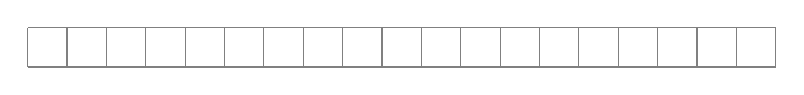
\begin{tikzpicture}
  \useasboundingbox (0,0) rectangle (9.5cm,0.5cm);
  \draw[step=0.5cm,color=gray] (0,0) grid (9.5cm,0.5cm);
\end{tikzpicture}}}}
% eine ganze Spalte Karos
\newcommand{\karospalte}{\null\leaders\karozeile\vskip 0pt plus 1fill\newpage}
\makeatletter
\newcommand{\notizenbisseitenende}{%
  % Spaltenumbruch, falls weniger als 4 cm Platz bleiben
  \par\ifdim\dimexpr\pagegoal-\pagetotal\relax<4cm\newpage\fi
  \subsection{Platz für eigene Notizen:}\par
  \leaders\karozeile\vskip 0pt plus 1fill
  \if@firstcolumn\newpage\null\leaders\karozeile\vskip 0pt plus 1fill\fi
  \clearpage
}
\makeatother
